\chapter{PCB}\label{ch:pcb}

\begin{flushright}{\slshape
    In which copper sheets are etched onto a red carpet\\
    connecting the different components together\\
    realizing their synergy and power
}
\end{flushright}

Disposition and explanation goes here. \TODO{Figure/image here too.}

\section {Introduction}

Design choices: \\
\subsection {Memory}
Since we decided to have separate instruction/data-memories, as well as VGA-ram, and
a dedicated memory for the AVR, we ended up with a total of 5 RAM-chips. The requirements
on the various chips did differ a bit though, we needed 8-bit words for all data, but
24 bit for instructions. Since 24-bit memory was out of production, and 32-bit memory
was too expensive, we opted for using two 16-bit chips, with their address-lines connected
together, and 8 ignored I/O-pins, thus in effect creating a 24-bit memory. Additionally,
as we were unsure about how constant we could get our data-streams, an additional
AVR-memory was added. This was chosen to be the same chip as the VGA-memory.

\subsection {VGA}
While we had a goal of creating our own VGA-controller in the FPGA, we decided to have
some fallback-option, thus, in addition to the neccessary pins and connectors for that
solution, we also added the necessary connectors for the VGA-module that Festina Lente
used last year.

\subsection {Communication}
We planned on using the SD-Card-reader as our main source of data/instructions, however
in the same vein as the design choices for the VGA, we opted to also have a fallback-solution
here, thus we also added USB and RS232 as fallback-solutions for getting data/communicating
with the computer.


%Flytta til process
%\subsection {Schematics}
The workflow of creating the schematic consisted of reading data sheets,
and looking at the reports from earlier computer design projects, and then
applying the knowledge we found from those to properly place the necessary
components in our schematic.

We decided to design the entire \ac{PCB} in one schematic, as the Festina Lente
report mentioned that Festina Lente-report does mention that 
``The decision to make the central components appear in multiple schematic
sheets made Altium issue a lot of warnings and errors during the design rule 
check''\cite[p.~49]{berg2011festinalente}. Something we avoided from day one, 
as we never attempted to use multiple schematics-documents.

A downside of this approach was the fact that this partially serialized
our work on the schematic, since we could not make concurrent changes to our
single document. When not working on the schematic, the other people in the
\ac{PCB} group did whatever could be done without touching the
schematic. (Making footprints, verifying design, looking up parts and data
sheets) Since the schematic was the biggest amount of work, this produced
something of a bottleneck for the PCB work.

However, having overall control of the entire thing in one document
did help to smooth out some issues we met while working. For instance,
we were having quite a few issues with net labels. This was quite easy to
solve when everything was in one document with no ports, as getting
complete overview was doable, without having to cross-reference schematics.
We also avoided the need to use any buses, although we did end up adding
some for the sake of readability.

The overall layout of the Schematic \ref{app:schematics} is logically grouped ``geographically'', to
allow for easy reading of the schematic.

\subsubsection {Buses/Wirelabels}
We initially worked from the assumption that all pins should be connected to a
bus, and then that bus should be connected to the pins in the other end. This
gave us some issues with duplicate naming. After digging through quite a bit of
Altium documentation, we became assured that simply wire-labeling the pins
would create the necessary connections. This is because any pin/wire with the
same name as any other pin/wire will be connected by definition in Altium.

This arguably made for a less readable schematic, as the bus-connected solution
was quite a lot easier to follow when tracing. However, as our schematic still
is logically grouped, it is not very hard to find the correct connections even
without the buses drawn in. We are quite sure that given a logical overview of
which components are directly connected to each other, finding the various pins
that perform this connection should be trivial even without the buses/wires
drawn in.

\section {Power supply}
\begin{figure}[h]
  \centering
  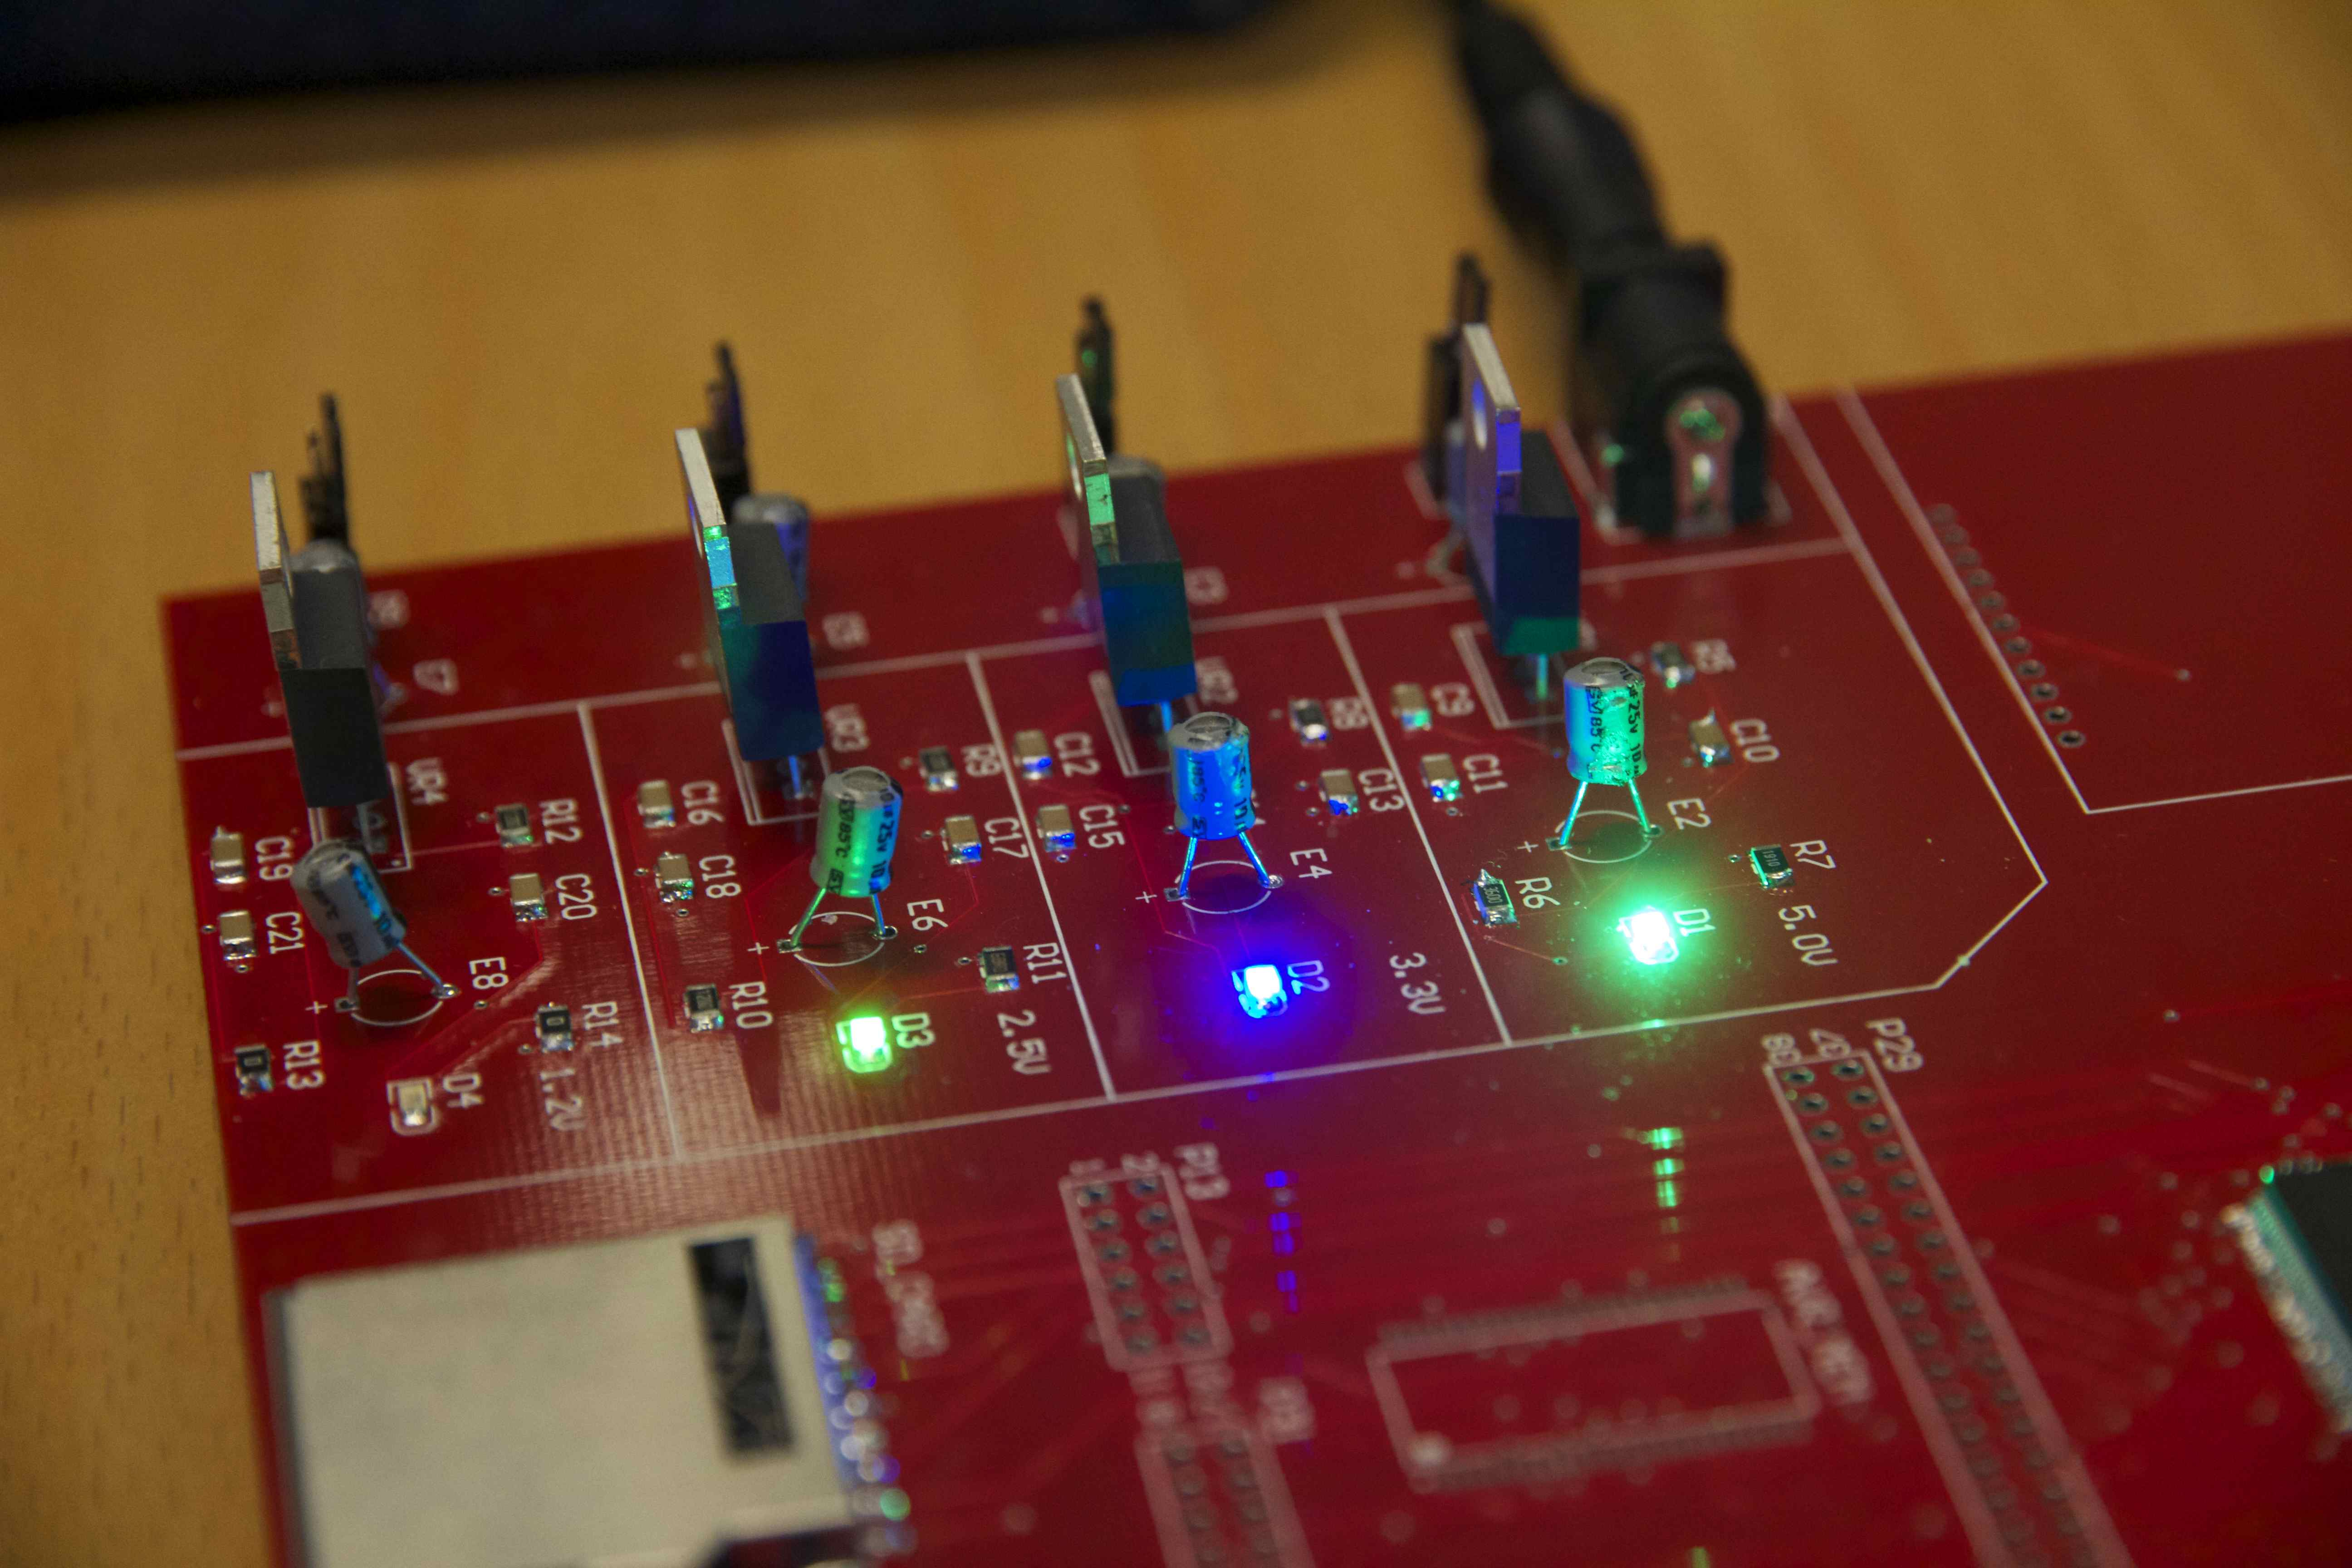
\includegraphics[width=0.8\textwidth]{fig/pcb/pcb_powersoldered.jpeg}
  \caption[The PCB Power Supply]{The PCB with the powersupply soldered.}
  \label{fig:pcb-powersoldered}
\end{figure}

After talking to Tufte and Jahre, we decided to reuse the power supply
from Festina Lente without any changes. Tufte said the power supply had evolved year by
year, and that it would therefore be a better solution to reuse it rather
than trying to create one from scratch. By doing so, we reduced the possibility 
of introducing new issues.

\section {Power plane}

\begin{figure}[h]
  \centering
  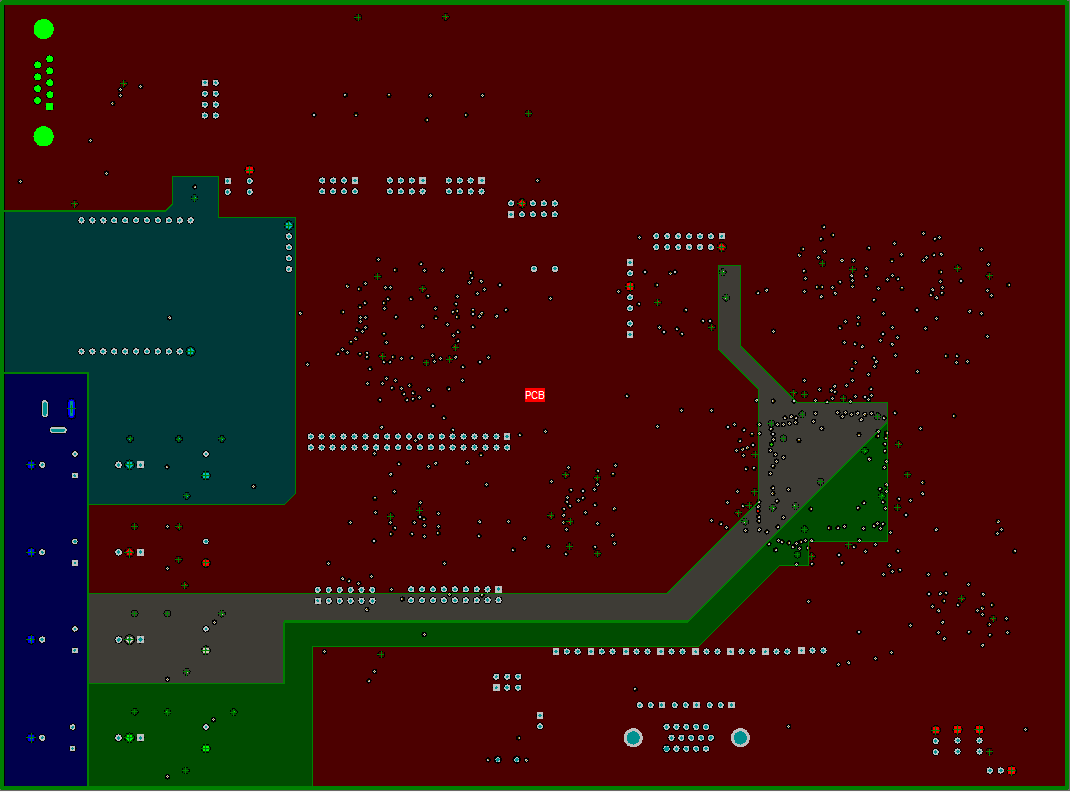
\includegraphics[width=0.8\textwidth]{fig/pcb/power_planes.PNG}
  \caption{The Power Planes}
  \label{fig:power_planes}
\end{figure}


Since our power supply was exactly the same as Festina Lente's we also ended up
with similar power planes, as seen on the figure above; 12V (dark blue), 5V (teal), 
3.3V (red), 2.5V (gray) and 1.2V (green). The 5V was only used for the external 
\ac{VGA} controller. 2.5V and 1.2V were split across the \ac{FPGA}.

The rest of the board got 3.3V. The entire power plane was put in internal layer
1, with a ground layer in internal layer 2.

\section {Footprints}
Some of the components we chose did not have footprints readily available, which
meant we either had to look for them on the internet, or create some ourselves.

This usually meant either staring at datasheets and carefully placing pins
relative to each other, or running the IPC-wizard.

\subsection {We made the following footprints ourselves}
\TODO{Make the links to references}
\begin {itemize}
\item SD-card \url{http://katalog.we-online.de/em/datasheet/693063010911.pdf}
  With the pin-designations selected by googling the pinouts for SD-cards in
  general, and comparing a few of those hits to make sure that the results
  agreed \url{http://pinouts.ru/Memory/sdcard_pinout.shtml} ended up being what
  we based the schematic-component based on. \CHECK{Mention that this was
    particularly hard to decipher from the datasheet, and that we did need to
    ask Gunnar for help at least once, just to read the datasheet?}
\item VGA-plug \url{http://www.te.com/commerce/DocumentDelivery/DDEController?Action=srchrtrv&DocNm=82068_AMPLIMITE_Right-Angle_Posted_Conn&DocType=Catalog+Section&DocLang=English&PartCntxt=}
\item Memory (TSOP54/TSOP44)
\TODO{Fill in a bit about the wizard used to generate this}
The TSOP54/TSOP44 footprints were created using the IPC Footprint Wizard, as
their datasheets fitted nicely with the Small Outline Package-setting in that
Wizard.

Data-memory (2M x 8bit) CY7C1069DV33 54TSOP:
\url{http://www.cypress.com/?docID=31945} Program-memory (64K x 16bit)
CY7C1021DV33 44TSOP: \url{http://www.cypress.com/?docID=31965} VGA memory (512 x
8bit) CY7C1049DV33 TSOP44 : \url{http://www.farnell.com/datasheets/1468461.pdf}
\end {itemize}

\subsection{Footprints from Festina Lente:}
As Festina Lente used some components that we also ended up using, we decided,
after talking to Gunnar\CHECK{Should we refer by first or last name?}, to use
their Footprints (as they were known good) for these components:
\url{http://org.ntnu.no/datamaskinerprosjekt2011/altium_libraries/dmprolibrary/}
\begin{itemize}
\item Button
\item Crystal
\item USB
\item Oscillator The oscillator had one issue last year, namely that the
  footprint was mirrored, noting this from Festina Lente's report, we read
  through the datasheet (REFERENCE)\TODO{Reference}, and remapped the
  pin-numbering on the foot-print before using this footprint.
\item PowerConnector
\item VGA-module
\end{itemize}
\CHECK{Molex? Still in the project, but wasn't used. Double-check this.}

In addition we used the following premade footprints:
\begin{itemize}
\item AVR-footprint | from AVR-freaks.
\item FPGA-footprint | Built-in from the Altium Designer Library.
\end{itemize}

\TODO{Mention the 1206-es that we chose to use based on the Festina
  Lente-report}

%Flytta til process
%\subsection {Routing}
\subsection {Routing}
\subsection {Routing}
\input{fig/pcb/routing}
We spent the entire final week before production working on the routing. In comparison, the energy group used only 2 days. There are quite a few possible reasons why we ended up using so much more time than them for this:

One of the reasons were simply that we were the first group to start routing. We thus got to fall into some gotcha-traps, with no one to warn us about them.

An example of such a trap was that we didn't set the correct Design Rules before auto-routing, until a few days into the week. This naturally didn't give us the routing that we wanted, and gave us a few headaches.

Related to this is the fact that we didn't experiment enough with different routing strategies. We wanted to reduce the number of vias, but went with the default routing in Altium. We then did quite an amount of manual routing to reduce the number of vias. Figure \ref{fig:removingvias-pcb} shows an example where we coupled together several pins to the same via going to the GND-layer. The amount of manual work could perhaps have been reduced by selecting the "Via Mixer" strategy instead.

\input{fig/pcb/pcb_removing_vias} \TODO{Write about this figure}

Another reason has to do with the difference between our designs. Where the other group had to route only 1 memory chip, we had 5. This naturally made the routing much more complex.

Initially we attempted auto routing. This took just around 12 minutes before constraints were set. And the better part of half an hour, after the constraints were set. This showed us quite a few issues that needed to be handled, and even more so when we finally got the constraints in.

\TODO{Fill in about the types of errors/warnings we got.}
\begin{itemize}
\item Constraints violations set wrong.
\item Power-plane net-labeled wrong.
\item Clearance constraints violated by Altium.
\item Short-circuiting vias.
\item Overlapping vias.
\item In general, the auto-routing started to produce violations.
\item more\ldots
\end{itemize}
\TODO{Silk-over-silk in USB/Lenna, errors we could ignore.}
\TODO{Scaling of board. (Should go elsewhere or not at all?)}

Initially we started with a board size chosen more or less at random, and picked something that seemed to fit the components comfortably with room to spare.

After laying out the components on the board, we noticed that the board had quite a bit of room left over. As this would be a waste of resources, we scaled the board down in size. We did this by moving the keep-out-borders inwards until the wasted space was removed, and then used the ``scale-to-fit-components''-tool in Altium, with the Keepout-border selected.

In the end we remapped some pins to increase physical proximity, and to untangle the amount of crossing wires. Although care was taken during this process, we accidentally happened to disconnect one pin in the schematic while reordering. We did notice this before production, and were able to correct the mistake by manually routing the connection. Finally, we did some manual routing to reduce the amount of unnecessary vias.


We spent the entire final week before production working on the routing. In comparison, the energy group used only 2 days. There are quite a few possible reasons why we ended up using so much more time than them for this:

One of the reasons were simply that we were the first group to start routing. We thus got to fall into some gotcha-traps, with no one to warn us about them.

An example of such a trap was that we didn't set the correct Design Rules before auto-routing, until a few days into the week. This naturally didn't give us the routing that we wanted, and gave us a few headaches.

Related to this is the fact that we didn't experiment enough with different routing strategies. We wanted to reduce the number of vias, but went with the default routing in Altium. We then did quite an amount of manual routing to reduce the number of vias. Figure \ref{fig:removingvias-pcb} shows an example where we coupled together several pins to the same via going to the GND-layer. The amount of manual work could perhaps have been reduced by selecting the "Via Mixer" strategy instead.

\begin{figure}[h]
  \centering
  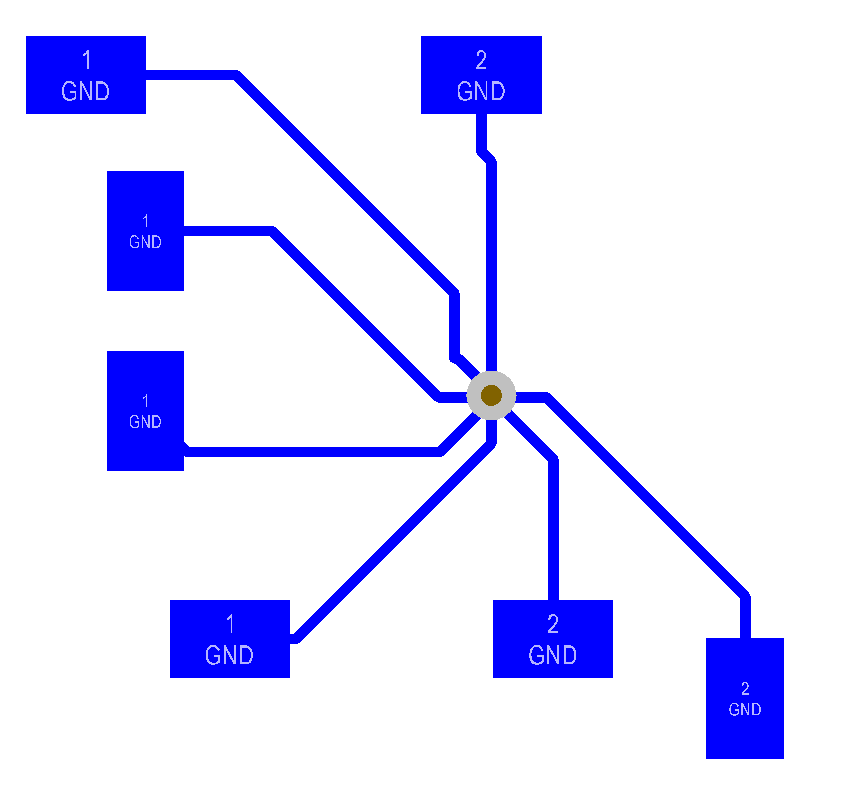
\includegraphics[width=0.8\textwidth]{fig/pcb/pcb_removing_vias.png}
  \caption{Removing vias}
  \label{fig:removingvias-pcb}
\end{figure}
 \TODO{Write about this figure}

Another reason has to do with the difference between our designs. Where the other group had to route only 1 memory chip, we had 5. This naturally made the routing much more complex.

Initially we attempted auto routing. This took just around 12 minutes before constraints were set. And the better part of half an hour, after the constraints were set. This showed us quite a few issues that needed to be handled, and even more so when we finally got the constraints in.

\TODO{Fill in about the types of errors/warnings we got.}
\begin{itemize}
\item Constraints violations set wrong.
\item Power-plane net-labeled wrong.
\item Clearance constraints violated by Altium.
\item Short-circuiting vias.
\item Overlapping vias.
\item In general, the auto-routing started to produce violations.
\item more\ldots
\end{itemize}
\TODO{Silk-over-silk in USB/Lenna, errors we could ignore.}
\TODO{Scaling of board. (Should go elsewhere or not at all?)}

Initially we started with a board size chosen more or less at random, and picked something that seemed to fit the components comfortably with room to spare.

After laying out the components on the board, we noticed that the board had quite a bit of room left over. As this would be a waste of resources, we scaled the board down in size. We did this by moving the keep-out-borders inwards until the wasted space was removed, and then used the ``scale-to-fit-components''-tool in Altium, with the Keepout-border selected.

In the end we remapped some pins to increase physical proximity, and to untangle the amount of crossing wires. Although care was taken during this process, we accidentally happened to disconnect one pin in the schematic while reordering. We did notice this before production, and were able to correct the mistake by manually routing the connection. Finally, we did some manual routing to reduce the amount of unnecessary vias.


We spent the entire final week before production working on the routing. In comparison, the energy group used only 2 days. There are quite a few possible reasons why we ended up using so much more time than them for this:

One of the reasons were simply that we were the first group to start routing. We thus got to fall into some gotcha-traps, with no one to warn us about them.

An example of such a trap was that we didn't set the correct Design Rules before auto-routing, until a few days into the week. This naturally didn't give us the routing that we wanted, and gave us a few headaches.

Related to this is the fact that we didn't experiment enough with different routing strategies. We wanted to reduce the number of vias, but went with the default routing in Altium. We then did quite an amount of manual routing to reduce the number of vias. Figure \ref{fig:removingvias-pcb} shows an example where we coupled together several pins to the same via going to the GND-layer. The amount of manual work could perhaps have been reduced by selecting the "Via Mixer" strategy instead.

\begin{figure}[h]
  \centering
  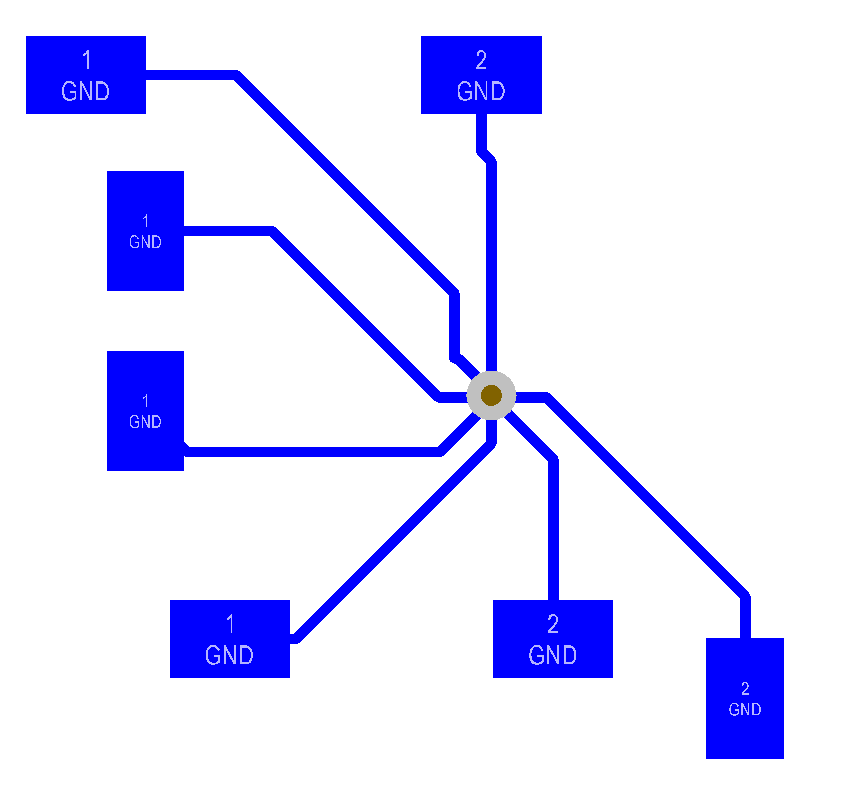
\includegraphics[width=0.8\textwidth]{fig/pcb/pcb_removing_vias.png}
  \caption{Removing vias}
  \label{fig:removingvias-pcb}
\end{figure}
 \TODO{Write about this figure}

Another reason has to do with the difference between our designs. Where the other group had to route only 1 memory chip, we had 5. This naturally made the routing much more complex.

Initially we attempted auto routing. This took just around 12 minutes before constraints were set. And the better part of half an hour, after the constraints were set. This showed us quite a few issues that needed to be handled, and even more so when we finally got the constraints in.

\TODO{Fill in about the types of errors/warnings we got.}
\begin{itemize}
\item Constraints violations set wrong.
\item Power-plane net-labeled wrong.
\item Clearance constraints violated by Altium.
\item Short-circuiting vias.
\item Overlapping vias.
\item In general, the auto-routing started to produce violations.
\item more\ldots
\end{itemize}
\TODO{Silk-over-silk in USB/Lenna, errors we could ignore.}
\TODO{Scaling of board. (Should go elsewhere or not at all?)}

Initially we started with a board size chosen more or less at random, and picked something that seemed to fit the components comfortably with room to spare.

After laying out the components on the board, we noticed that the board had quite a bit of room left over. As this would be a waste of resources, we scaled the board down in size. We did this by moving the keep-out-borders inwards until the wasted space was removed, and then used the ``scale-to-fit-components''-tool in Altium, with the Keepout-border selected.

In the end we remapped some pins to increase physical proximity, and to untangle the amount of crossing wires. Although care was taken during this process, we accidentally happened to disconnect one pin in the schematic while reordering. We did notice this before production, and were able to correct the mistake by manually routing the connection. Finally, we did some manual routing to reduce the amount of unnecessary vias.


\section {PCB testing}

\begin{figure}[h]
  \centering
  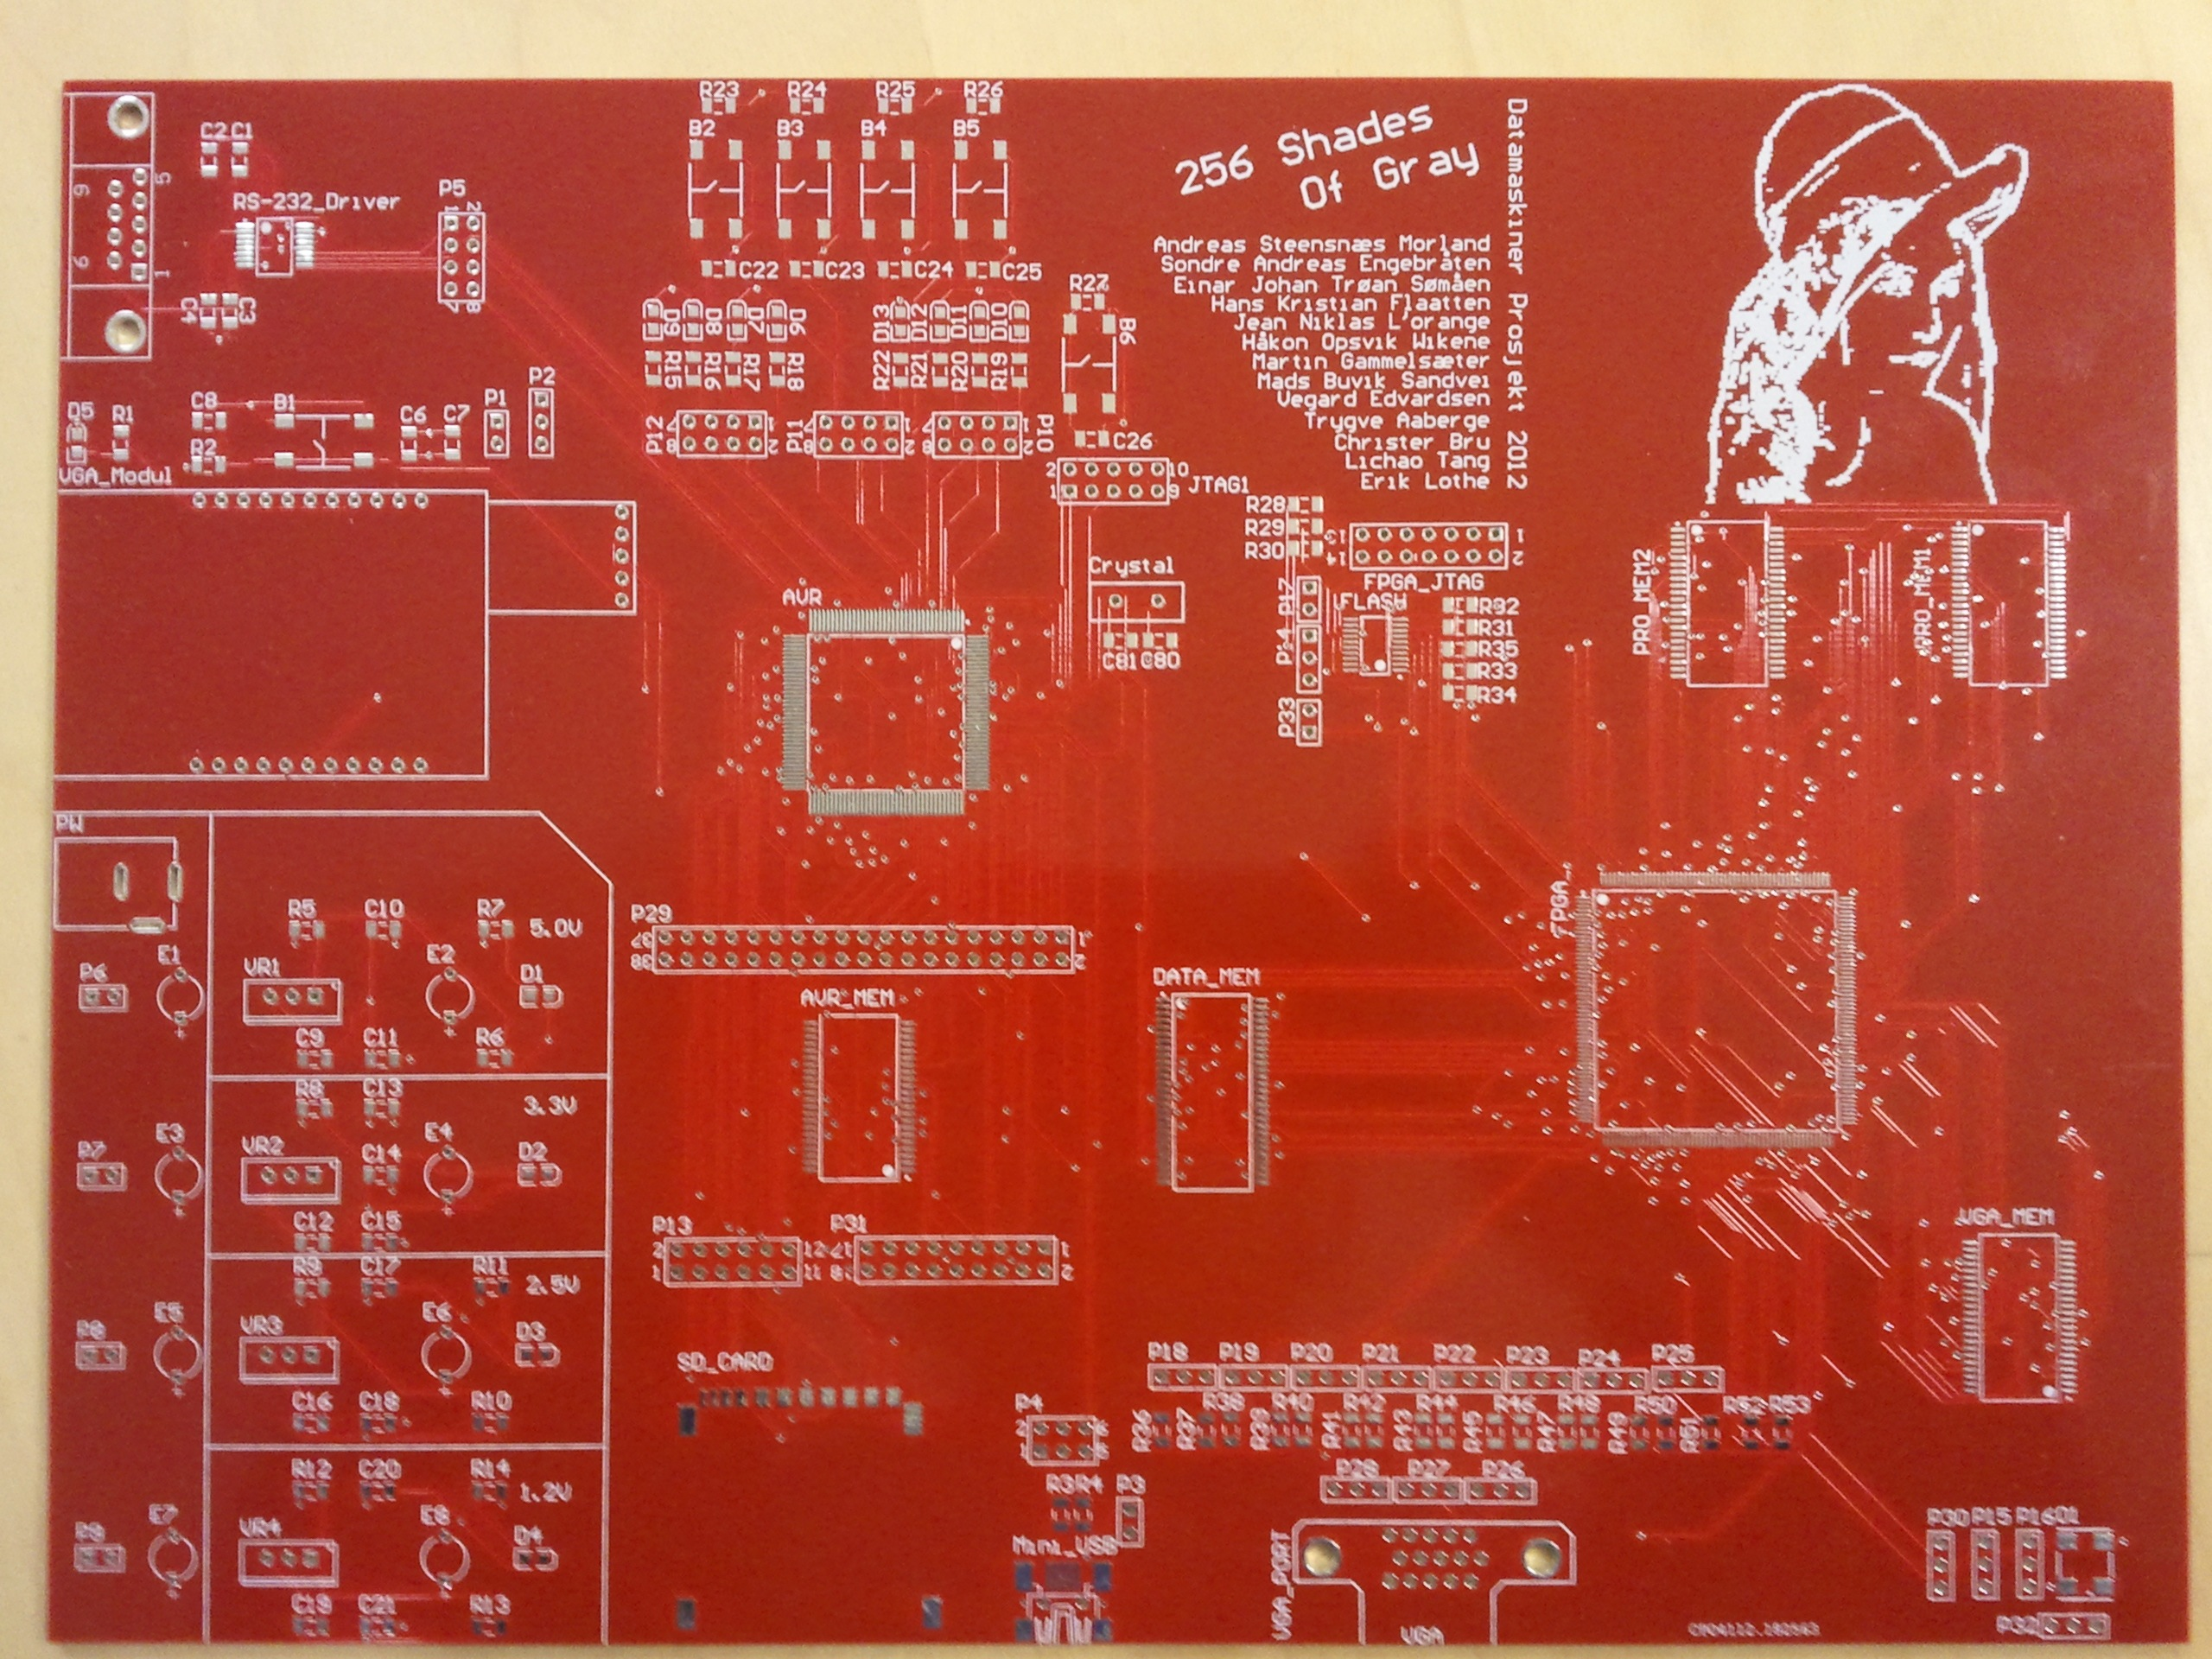
\includegraphics[width=0.8\textwidth]{fig/pcb/pcbwithoutcomp.jpg}
  \caption{The PCB Without Components}
  \label{fig:pcb-without-components}
\end{figure}


When the \ac{PCB} arrived from production, the soldering proved
to be a bit more difficult than originally anticipated.
First, we tested whether
there were any short circuits in the board itself. We used the multimeter to test that
there was no current passing from one layer to another. Then, we started to solder the power supply, one power plane at time, testing the board for short
circuit after each iteration. The table \ref{fig:pcb} shows the observed voltage from each plane.

\begin{table}[h]
  \centering
  \begin{tabularx}{\textwidth}{l l l l}\toprule
    \thx{Test} & \thx{Result} & \thx{Passed} 
    \\ 
	 \midrule
    Power supply 12.0V               &Measured 12.045  & OK  \\	
\midrule
    Power supply 5.0V               &Measured 4.995  & OK  \\
    \midrule
    Power supply 3.3V                   & Measured 3.286 & OK  \\
    \midrule
    Power supply 2.5V                 & Measured 2.510 & OK \\
    \midrule
    Power supply 1.2V            & Measured 1.240 & OK  \\
    
    \bottomrule
  \end{tabularx}
  \caption{Results of power supply}
  \label{fig:pcb}
\end{table}


\begin{figure}[h]
  \centering
  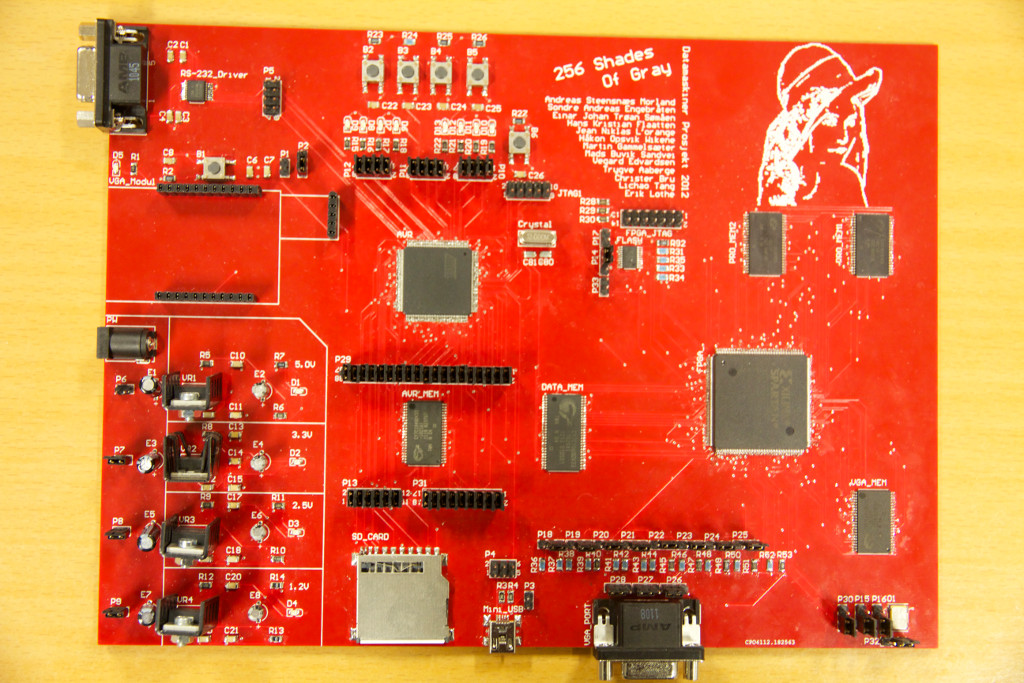
\includegraphics[width=0.8\textwidth]{fig/pcb/pcbwithcompnew.jpeg}
  \caption[The PCB]{The PCB With All The Components.}
  \label{fig:pcb-with-components}
\end{figure}


\section {Process}
This section describes the work and design challenges faced related to the PCB.
\subsection{Memory}
As discussed earlier, as one of our earliest design choices we chose 3 separate memories to allow overlap of
memory accesses. Since the requirements for the data/instruction memories differed in both size and word-width 
we wound up with not only separate, but also different chips for this purpose. The same choice meant we also
needed a separate memory for our \ac{VGA} controller, as that needed to read it's buffer as fast as possible
without interfering with the speed of the rest of the system. This called for a memory that was big enough to
hold atleast a full screen-frame, at 8-bit per pixel (since each pixel is an 8-bit greyscale pixel).

To reduce the possibility of having too slow data-access from the AVR, an extra memory was added to work as
a buffer for the AVR as well. This design choice was made {\em after} ordering, which meant that we had to choose from
the chips we had already ordered to fit this purpose. Since this was intended to carry data intended for the rest
of the system, and as the rest of the system is working with data in 8-bit bytes, we ended up using one of the
extra chips ordered as \ac{VGA} memory for this purpose.

\subsection {Schematics}
The workflow of creating the schematic consisted of reading data sheets,
and looking at the reports from earlier computer design projects, and then
applying the knowledge we found from those to properly place the necessary
components in our schematic.

We decided to design the entire \ac{PCB} in one schematic, as the Festina Lente
report mentioned that Festina Lente-report does mention that 
``The decision to make the central components appear in multiple schematic
sheets made Altium issue a lot of warnings and errors during the design rule 
check''\cite[p.~49]{berg2011festinalente}. Something we avoided from day one, 
as we never attempted to use multiple schematics-documents.

A downside of this approach was the fact that this partially serialized
our work on the schematic, since we could not make concurrent changes to our
single document. When not working on the schematic, the other people in the
\ac{PCB} group did whatever could be done without touching the
schematic. (Making footprints, verifying design, looking up parts and data
sheets) Since the schematic was the biggest amount of work, this produced
something of a bottleneck for the PCB work.

However, having overall control of the entire thing in one document
did help to smooth out some issues we met while working. For instance,
we were having quite a few issues with net labels. This was quite easy to
solve when everything was in one document with no ports, as getting
complete overview was doable, without having to cross-reference schematics.
We also avoided the need to use any buses, although we did end up adding
some for the sake of readability.

The overall layout of the Schematic \ref{app:schematics} is logically grouped ``geographically'', to
allow for easy reading of the schematic.

\subsubsection {Buses/Wirelabels}
We initially worked from the assumption that all pins should be connected to a
bus, and then that bus should be connected to the pins in the other end. This
gave us some issues with duplicate naming. After digging through quite a bit of
Altium documentation, we became assured that simply wire-labeling the pins
would create the necessary connections. This is because any pin/wire with the
same name as any other pin/wire will be connected by definition in Altium.

This arguably made for a less readable schematic, as the bus-connected solution
was quite a lot easier to follow when tracing. However, as our schematic still
is logically grouped, it is not very hard to find the correct connections even
without the buses drawn in. We are quite sure that given a logical overview of
which components are directly connected to each other, finding the various pins
that perform this connection should be trivial even without the buses/wires
drawn in.


\subsection {Routing}
\subsection {Routing}
\subsection {Routing}
\input{fig/pcb/routing}
We spent the entire final week before production working on the routing. In comparison, the energy group used only 2 days. There are quite a few possible reasons why we ended up using so much more time than them for this:

One of the reasons were simply that we were the first group to start routing. We thus got to fall into some gotcha-traps, with no one to warn us about them.

An example of such a trap was that we didn't set the correct Design Rules before auto-routing, until a few days into the week. This naturally didn't give us the routing that we wanted, and gave us a few headaches.

Related to this is the fact that we didn't experiment enough with different routing strategies. We wanted to reduce the number of vias, but went with the default routing in Altium. We then did quite an amount of manual routing to reduce the number of vias. Figure \ref{fig:removingvias-pcb} shows an example where we coupled together several pins to the same via going to the GND-layer. The amount of manual work could perhaps have been reduced by selecting the "Via Mixer" strategy instead.

\input{fig/pcb/pcb_removing_vias} \TODO{Write about this figure}

Another reason has to do with the difference between our designs. Where the other group had to route only 1 memory chip, we had 5. This naturally made the routing much more complex.

Initially we attempted auto routing. This took just around 12 minutes before constraints were set. And the better part of half an hour, after the constraints were set. This showed us quite a few issues that needed to be handled, and even more so when we finally got the constraints in.

\TODO{Fill in about the types of errors/warnings we got.}
\begin{itemize}
\item Constraints violations set wrong.
\item Power-plane net-labeled wrong.
\item Clearance constraints violated by Altium.
\item Short-circuiting vias.
\item Overlapping vias.
\item In general, the auto-routing started to produce violations.
\item more\ldots
\end{itemize}
\TODO{Silk-over-silk in USB/Lenna, errors we could ignore.}
\TODO{Scaling of board. (Should go elsewhere or not at all?)}

Initially we started with a board size chosen more or less at random, and picked something that seemed to fit the components comfortably with room to spare.

After laying out the components on the board, we noticed that the board had quite a bit of room left over. As this would be a waste of resources, we scaled the board down in size. We did this by moving the keep-out-borders inwards until the wasted space was removed, and then used the ``scale-to-fit-components''-tool in Altium, with the Keepout-border selected.

In the end we remapped some pins to increase physical proximity, and to untangle the amount of crossing wires. Although care was taken during this process, we accidentally happened to disconnect one pin in the schematic while reordering. We did notice this before production, and were able to correct the mistake by manually routing the connection. Finally, we did some manual routing to reduce the amount of unnecessary vias.


We spent the entire final week before production working on the routing. In comparison, the energy group used only 2 days. There are quite a few possible reasons why we ended up using so much more time than them for this:

One of the reasons were simply that we were the first group to start routing. We thus got to fall into some gotcha-traps, with no one to warn us about them.

An example of such a trap was that we didn't set the correct Design Rules before auto-routing, until a few days into the week. This naturally didn't give us the routing that we wanted, and gave us a few headaches.

Related to this is the fact that we didn't experiment enough with different routing strategies. We wanted to reduce the number of vias, but went with the default routing in Altium. We then did quite an amount of manual routing to reduce the number of vias. Figure \ref{fig:removingvias-pcb} shows an example where we coupled together several pins to the same via going to the GND-layer. The amount of manual work could perhaps have been reduced by selecting the "Via Mixer" strategy instead.

\begin{figure}[h]
  \centering
  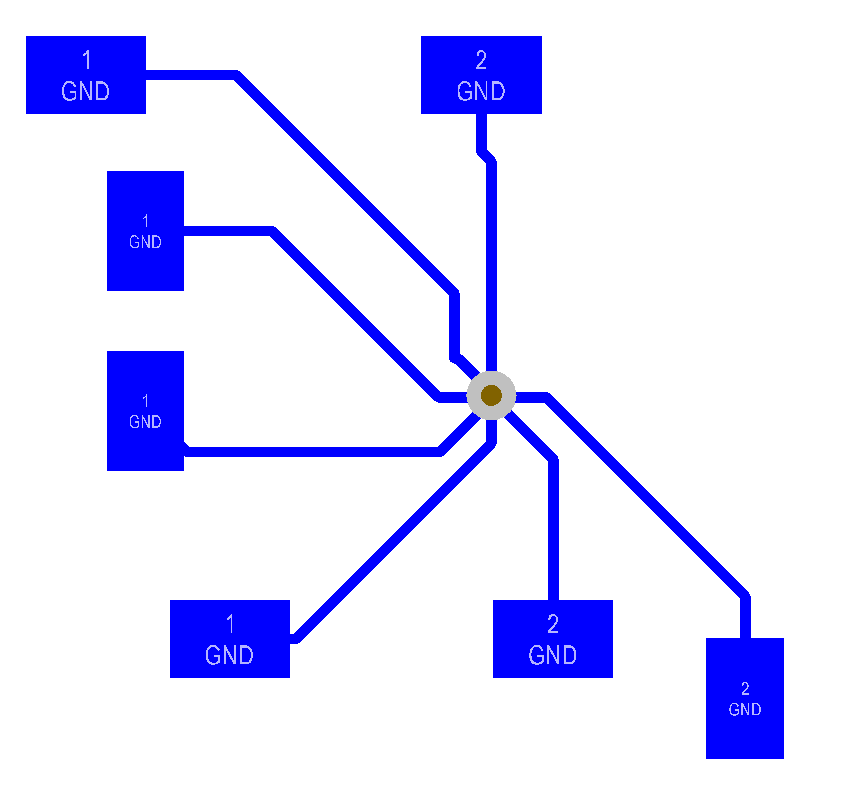
\includegraphics[width=0.8\textwidth]{fig/pcb/pcb_removing_vias.png}
  \caption{Removing vias}
  \label{fig:removingvias-pcb}
\end{figure}
 \TODO{Write about this figure}

Another reason has to do with the difference between our designs. Where the other group had to route only 1 memory chip, we had 5. This naturally made the routing much more complex.

Initially we attempted auto routing. This took just around 12 minutes before constraints were set. And the better part of half an hour, after the constraints were set. This showed us quite a few issues that needed to be handled, and even more so when we finally got the constraints in.

\TODO{Fill in about the types of errors/warnings we got.}
\begin{itemize}
\item Constraints violations set wrong.
\item Power-plane net-labeled wrong.
\item Clearance constraints violated by Altium.
\item Short-circuiting vias.
\item Overlapping vias.
\item In general, the auto-routing started to produce violations.
\item more\ldots
\end{itemize}
\TODO{Silk-over-silk in USB/Lenna, errors we could ignore.}
\TODO{Scaling of board. (Should go elsewhere or not at all?)}

Initially we started with a board size chosen more or less at random, and picked something that seemed to fit the components comfortably with room to spare.

After laying out the components on the board, we noticed that the board had quite a bit of room left over. As this would be a waste of resources, we scaled the board down in size. We did this by moving the keep-out-borders inwards until the wasted space was removed, and then used the ``scale-to-fit-components''-tool in Altium, with the Keepout-border selected.

In the end we remapped some pins to increase physical proximity, and to untangle the amount of crossing wires. Although care was taken during this process, we accidentally happened to disconnect one pin in the schematic while reordering. We did notice this before production, and were able to correct the mistake by manually routing the connection. Finally, we did some manual routing to reduce the amount of unnecessary vias.


We spent the entire final week before production working on the routing. In comparison, the energy group used only 2 days. There are quite a few possible reasons why we ended up using so much more time than them for this:

One of the reasons were simply that we were the first group to start routing. We thus got to fall into some gotcha-traps, with no one to warn us about them.

An example of such a trap was that we didn't set the correct Design Rules before auto-routing, until a few days into the week. This naturally didn't give us the routing that we wanted, and gave us a few headaches.

Related to this is the fact that we didn't experiment enough with different routing strategies. We wanted to reduce the number of vias, but went with the default routing in Altium. We then did quite an amount of manual routing to reduce the number of vias. The amount of manual work could perhaps have been reduced by selecting the "Via Mixer" strategy instead.

\TODO{Insert "via-hub" figure here}

Another reason has to do with the difference between our designs. Where the other group had to route only 1 memory chip, we had 5. This naturally made the routing much more complex.

Initially we attempted autorouting. This took just around 12 minutes before constraints were set. And the better part of half an hour, after the constraints were set. This showed us quite a few issues that needed to be handled, and even more so when we finally got the constraints in.

\TODO{Fill in about the types of errors/warnings we got.}
\begin{itemize}
\item Constraints violations set wrong.
\item Power-plane net-labeled wrong.
\item Clearance constraints violated by Altium.
\item Short-circuiting vias.
\item Overlapping vias.
\item In general, the auto-routing started to produce violations.
\item more\ldots
\end{itemize}
\TODO{Silk-over-silk in USB/Lenna, errors we could ignore.}
\TODO{Scaling of board. (Should go elsewhere or not at all?)}

Initially we started with a board size chosen more or less at random, and picked something that seemed to fit the components comfortably with room to spare.

After laying out the components on the board, we noticed that the board had quite a bit of room left over. As this would be a waste of resources, we scaled the board down in size. We did this by moving the keep-out-borders inwards until the wasted space was removed, and then used the ``scale-to-fit-components''-tool in Altium, with the Keepout-border selected.

In the end we remapped some pins to increase physical proximity, and to untangle the amount of crossing wires. Although care was taken during this process, we accidentally happened to disconnect one pin in the schematic while reordering. We did notice this before production, and were able to correct the mistake by manually routing the connection. Finally, we did some manual routing to reduce the amount of unneccessary vias.

\subsection{Soldering}
After that we started soldering the AVR. Getting the AVR in place was particularly difficult,
but after asking Tufte, we lent a glue stick to put some glue on. The increased friction helped keeping the AVR in place during soldering.

After about a days work we managed to completely destroy a pin on the AVR,
therefore we had to start from scratch on a new board. On this new board we
started with the AVR and \ac{FPGA}, as they were the hardest components to
solder. After each side on the AVR and \ac{FPGA}, we tested for short
circuits. As none were found, we moved on to the power supply, as well as
\acp{JTAG}, FLASH and \acp{LED}. In order to check the \ac{PCB} was working, the
AVR and \ac{FPGA} groups tested the \ac{PCB} board without the capacitors, after
both groups tested that they could connect to the AVR and \ac{FPGA}
respectively, we began to solder the rest part of the \ac{PCB}.


\section {Problems and Workarounds}
\subsection{Routing}
Routing was the first problem we confronted during the designing the \ac{PCB}
board, we had to manually route the design, because we got some warnings due to
the clearance of the board. We used the auto-routing function provided by
Altium, yet as it did not provide satisfying results, we tried to change some
parameters to make them better, without success. Finally, we realized that we
had to route a few wires manually. This was mostly motivated by our desire to
not have vias as close to the pins as Altium placed them. Also, as to cut down
the budget, we removed some unnecessary vias by wiring multiple grounds and
powers together, where the design allowed us to. In this way, we got quite a few
less vias.

We spent the entire final week before production working on the routing. In comparison, the energy group used only 2 days. There are quite a few possible reasons why we ended up using so much more time than them for this:

One of the reasons were simply that we were the first group to start routing. We thus had no one to warn us about mistakes. An example of such a mistake was that we did not set the correct Design Rules before auto-routing, until a few days into the week. This naturally did not give us the routing that we wanted, and gave us a few headaches.

Related to this is the fact that we did not experiment enough with different routing strategies.

Another reason relates to the difference between our designs. Where the other group had to route only 1 memory chip, we had 5. This naturally made the routing much more complex.
\subsection{Soldering}
Soldering was the biggest problem that we faced, none of the \ac{PCB} group
member had any experiences with it beforehand. We managed to destroy our first
board, as we used too much tin on one of the AVR pins, and ruined them by using
the tin removal unit wrongly.

The next try, however, proved to be successful, but there still remained some
minor problems. Problems we found were lack of tin on the oscillator, as well as
a few of the \ac{FPGA} pins. They were, as opposed to our problem with the first
board, easily fixed, once discovered.



